\documentclass[12pt]{report} 

%load any additional packages
\usepackage{amssymb}
\usepackage{amsfonts}
\usepackage{graphicx}
\usepackage{natbib}
\usepackage{multicol}
\usepackage{float}
\usepackage{tikz}
\usetikzlibrary{positioning, arrows.meta, shapes.geometric}
\usepackage{amsmath}
\usepackage{booktabs}
\usepackage[colorlinks=true,linkcolor=blue,citecolor=blue,urlcolor=cyan]{hyperref}
\usepackage{verbatim}
\usepackage{listings}
\usepackage{xcolor}

\lstset{
  basicstyle=\ttfamily\small,
  breaklines=true,
  frame=single,
  backgroundcolor=\color{gray!10},
  keywordstyle=\color{blue},
  commentstyle=\color{green!50!black},
  stringstyle=\color{red!60!black},
}

\setlength{\topmargin}{0.0in}
\setlength{\oddsidemargin}{0.33in}
\setlength{\evensidemargin}{-0.08in}
\setlength{\textheight}{8.5in}
\setlength{\textwidth}{6.0in}

\def\mytitle{Small Language Models for Marine Hydrodynamics Problem Solving using RLPT}
\def\myname{Raghuveer Patil}
\def\mydegree{Master of Technology}
\def\mysupervisor{Prof. Prabhat Kumar Mishra}
\def\myrollno{21NA3AI42}
\def\mydep{Department of Artificial Intelligence}
\def\mydegreedate{24th April, 2026}

\begin{document}
 \baselineskip=18pt plus1pt
 \setcounter{secnumdepth}{3}
 \setcounter{tocdepth}{3}
 \pagenumbering{roman}
 
% =============================================================================
% TITLE PAGE
% =============================================================================
\begin{titlepage}
\begin{center}

\vspace*{1cm}

{\Large \textbf{Small Language Models for Marine Hydrodynamics Problem Solving using RLPT}}

\vspace{1.5cm}

{\large \textit{Thesis to be submitted in the partial fulfillment of the requirements for the degree}}

\vspace{0.8cm}

{\large \textbf{MASTER OF TECHNOLOGY}}

\vspace{0.3cm}

{\large IN}

\vspace{0.3cm}

{\large \textbf{ARTIFICIAL INTELLIGENCE}}

\vspace{0.8cm}

{\large by}

\vspace{0.5cm}

{\Large \textbf{Raghuveer Patil}}

{\large (21NA3AI42)}

\vspace{1.0cm}

{\large Under the guidance of}

\vspace{0.5cm}

{\Large \textbf{Prof. Prabhat Kumar Mishra}}

\vspace{1.5cm}

% ---- IIT KGP LOGO PLACEHOLDER ----
% Uncomment the following line and provide the path to the IIT KGP logo:
% \includegraphics[width=3cm]{iitk_logo.png}
\vspace{1.0cm}
% ---- END LOGO PLACEHOLDER ----

{\large Department of Artificial Intelligence}\\
{\large Indian Institute of Technology, Kharagpur}\\
{\large 24th April, 2026}

\end{center}
\end{titlepage}

% =============================================================================
% CERTIFICATE
% =============================================================================
\newpage
\thispagestyle{plain}
\begin{center}
{\large \textbf{Department of Artificial Intelligence}}\\
{\large \textbf{Indian Institute of Technology,}}\\
{\large \textbf{Kharagpur}}\\
{\large India -- 721302}
\end{center}

\vspace{1.5cm}

\begin{center}
{\Large \textbf{CERTIFICATE}}
\end{center}

\vspace{1cm}

This is to certify that we have examined the thesis entitled \textbf{Small Language Models for Marine Hydrodynamics Problem Solving using RLPT}, submitted by \textbf{Raghuveer Patil} (Roll Number: 21NA3AI42) a postgraduate student of Department of Artificial Intelligence in partial fulfillment for the award of degree of Master of Technology. We hereby accord our approval of it as a study carried out and presented in a manner required for its acceptance in partial fulfillment for the Post Graduate Degree for which it has been submitted. The thesis has fulfilled all the requirements as per the regulations of the Institute and has reached the standard needed for submission.

\vspace{3cm}

\noindent
\textbf{Supervisor}\\
Department of Artificial Intelligence\\
Indian Institute of Technology, Kharagpur

\vspace{1.5cm}

\noindent
Place: Kharagpur\\
Date:

\clearpage

% =============================================================================
% ACKNOWLEDGEMENTS
% =============================================================================
\chapter*{Acknowledgements}
\addcontentsline{toc}{chapter}{Acknowledgements}

I would like to express my deepest gratitude to my supervisor, Prof. Prabhat Kumar Mishra, who introduced me to the exciting intersection of Reinforcement Learning and domain-specific language modelling. His profound expertise and insightful guidance have been instrumental in the progress and success of my research. I am also indebted to the faculty and staff of the Department of Artificial Intelligence, whose assistance has been invaluable throughout my academic journey. Their willingness to share knowledge and offer advice has greatly enriched my learning experience. Special thanks are due to my peers and colleagues who have provided me with support and collaboration. Their perspectives and feedback have been a source of encouragement and growth. Finally, and most importantly, my heartfelt thanks go to my family. Their unwavering support, endless patience, and belief in my abilities have been my strength and perseverance. This accomplishment is as much theirs as it is mine.

% =============================================================================
% ABSTRACT
% =============================================================================
\chapter*{Abstract}
\addcontentsline{toc}{chapter}{Abstract}

Recent advances in Large Language Models (LLMs) have demonstrated remarkable capabilities in general-purpose reasoning, yet these models frequently underperform on specialized engineering tasks requiring structured numerical reasoning and domain-specific knowledge. This thesis investigates the central question of whether GRPO-based RL post-training can bring a Small Language Model (SLM) to frontier LLM performance levels on domain-specific engineering problems --- specifically, whether a 3-billion-parameter model fine-tuned on marine hydrodynamics can match or exceed a general-purpose frontier LLM on the same evaluation set.

We propose a multi-stage pipeline comprising synthetic dataset generation, Supervised Fine-Tuning (SFT), and GRPO-based RL post-training via Group Relative Policy Optimization (GRPO). Source materials comprise the marine hydrodynamics textbooks of \citet{newman1977marine,faltinsen1993sea}; MIT OpenCourseWare courses 2.20 and 2.29 \citep{mitocw220,mitocw229}, taught respectively by Prof.\ Dick K.~P.~Yue and Prof.\ Jerome H.~Milgram; and graduate examination papers for IIT Kharagpur subject NA20202 \citep{iitkgp_na20202_exams}. These are processed through a text-extraction and OCR pipeline to produce approximately 563 text chunks. A synthetic question--answer generation system powered by the Groq API (LLaMA~3.3~70B) produces approximately 2,750 QA pairs spanning conceptual, numerical, and multiple-choice question types, each accompanied by a Chain-of-Thought reasoning trace.

The SFT stage fine-tunes a \texttt{Qwen2.5-3B-Instruct} model using LoRA adapters on an NVIDIA H100 NVL GPU. A significant debugging effort was required to resolve persistent NaN gradient failures traced to BF16 precision accumulation errors across multiple LoRA target modules. The final SFT model achieves a training loss of 0.9729 and evaluation token accuracy of 77.43\%.

The GRPO stage introduces a physics-based reward function combining numerical correctness verification (via SymPy), MCQ letter-matching, and a format reward to ensure non-zero intra-group advantage variance. Across five GRPO training runs --- incorporating progressively refined reward functions, a clean data pipeline (SFT-2), a critical \texttt{max\_new\_tokens} fix, and expanded LoRA capacity --- numerical accuracy improves from 27.60\% (leak-free SFT-2 baseline) to 38.91\%, and MCQ accuracy improves from 71.82\% to 85.45\%. Critical implementation challenges including the zero-gradient problem, TRL API incompatibilities, and a truncation bug corrupting the reward signal are documented and resolved.

To contextualise performance, the evaluation set is also presented to a frontier LLM (Gemini) via its web interface. The domain-fine-tuned SLM achieves \textbf{38.91\% numerical accuracy} and \textbf{80.00\% MCQ accuracy}, compared to Gemini's 37.10\% and 78.18\% respectively --- demonstrating that GRPO-based RL post-training successfully brings the SLM to and slightly beyond frontier LLM performance on this domain-specific benchmark. Both models exhibit an identical formula-selection failure pattern, confirming that the remaining accuracy ceiling is a data representation limitation rather than a model capacity issue.

% =============================================================================
% TABLE OF CONTENTS AND LISTS
% =============================================================================
\tableofcontents
\listoffigures
\listoftables

% =============================================================================
% MAIN MATERIAL
% =============================================================================
\clearpage
\pagenumbering{arabic}


% %%%%%%%%%%%%%%%%%%%%%%%%%%%%%%%%%%%%%%%%%%%%%%%%%%%%%%%%%%%%%%%%%%%%%%%%%%%%%
% CHAPTER 1: INTRODUCTION
% %%%%%%%%%%%%%%%%%%%%%%%%%%%%%%%%%%%%%%%%%%%%%%%%%%%%%%%%%%%%%%%%%%%%%%%%%%%%%
\chapter{Introduction}

\section{Background}

Recent developments in Large Language Models (LLMs) have demonstrated remarkable capabilities in reasoning, coding, and natural language understanding. Models with hundreds of billions of parameters can perform sophisticated multi-step reasoning and generate coherent, contextually appropriate responses across diverse domains. However, these models are computationally expensive and often inefficient for domain-specific tasks requiring structured numerical reasoning and deep subject-matter expertise.

Recent research indicates that Small Language Models (SLMs) with 1--8 billion parameters, when fine-tuned on specialized datasets, can match or outperform larger models on specific tasks while requiring significantly lower computational resources \citep{slm_survey2025}. Surveys of recent work confirm that task-specific SLMs frequently rival or exceed larger models on focused benchmarks such as reasoning, structured output generation, and domain-specific question answering \citep{redhat_slm2024}.

This thesis explores the use of SLMs trained with GRPO-based RL post-training to solve marine hydrodynamics problems. The \textbf{central goal} is to determine whether a small model with 3 billion parameters can be brought to frontier LLM performance levels on domain-specific hydrodynamics questions through GRPO-based RL post-training --- leveraging synthetic dataset generation and physics-based reward verification to enable reinforcement learning in a data-scarce domain. This is motivated by the broader question in the field: can GRPO-based RL post-training compensate for the knowledge gap between a small fine-tuned model and a much larger general-purpose LLM?

\section{Problem Statement}

Hydrodynamics is a specialised engineering domain involving problems related to potential flow theory, wave--body interactions, ship hydrodynamics, boundary layer theory, and fluid forces and hydrodynamic coefficients. While general-purpose LLMs possess broad knowledge, they often perform poorly on specialised engineering problems requiring structured reasoning and equation-based solutions.

Three key challenges motivate this work:

\begin{enumerate}
    \item \textbf{Lack of labelled datasets:} Very few publicly available question--answer datasets exist for marine hydrodynamics. Unlike natural language understanding or code generation, this domain has no established benchmark.
    
    \item \textbf{Requirement for numerical and symbolic reasoning:} Many problems require equation derivations, numerical calculations, and multi-step reasoning that go beyond pattern matching.
    
    \item \textbf{Evaluation difficulty:} Solutions must be verified using physical laws and equations rather than subjective evaluation, necessitating automated physics-based verification.
\end{enumerate}

This thesis investigates whether a domain-specialised SLM trained using reinforcement learning with verifiable physics-based rewards can solve hydrodynamics problems more accurately than general-purpose approaches.

\section{Research Objectives}

The primary objectives of this project are:

\begin{enumerate}
    \item \textbf{To develop a task-specific Small Language Model} for marine hydrodynamics problem solving.
    
    \item \textbf{To create a hydrodynamics dataset} using synthetic data generation techniques from the textbooks and open course materials cited in Section~\ref{sec:source_materials}.
    
    \item \textbf{To design a physics-based reward verification system} for reinforcement learning that combines numerical comparison, symbolic equivalence checking, and structural format verification.
    
    \item \textbf{To train the model using Supervised Fine-Tuning (SFT) followed by GRPO-based RL post-training}, establishing a complete two-stage alignment pipeline.
    
    \item \textbf{To evaluate whether GRPO-based RL post-training can bring the SLM to frontier LLM performance levels} by comparing the final model against a general-purpose LLM (Gemini) on the same held-out evaluation set.
    
    \item \textbf{To document the complete engineering process}, including all debugging challenges, failure modes, and their resolutions, to aid reproducibility.
\end{enumerate}

\section{Contributions}

This thesis makes the following contributions:

\begin{itemize}
    \item \textbf{Marine Hydrodynamics QA Dataset:} A synthetic dataset of approximately 2,750 question--answer pairs with Chain-of-Thought reasoning, spanning conceptual, numerical, and multiple-choice question types, generated from the textbooks of \citet{newman1977marine,faltinsen1993sea}, MIT OpenCourseWare materials \citep{mitocw220,mitocw229}, and IIT Kharagpur NA20202 examination papers \citep{iitkgp_na20202_exams}.
    
    \item \textbf{Domain-Specific SLM Training Pipeline:} A complete, reproducible pipeline from text extraction and OCR through synthetic QA generation, SFT, and GRPO training, all operating on a single GPU server.
    
    \item \textbf{Physics-Grounded Reward Function:} A multi-component reward function for GRPO that combines numerical correctness verification (with graded partial credit), MCQ letter-matching, and format rewards to ensure effective policy gradient training.
    
    \item \textbf{Detailed Error Analysis:} Comprehensive documentation of critical debugging challenges including BF16 NaN gradient failures, TRL API incompatibilities, the GRPO zero-gradient problem, and a truncation bug affecting reward signals.
    
    \item \textbf{Empirical Results:} Evidence that five GRPO training runs improve numerical accuracy from 27.60\% to 38.91\% and MCQ accuracy from 71.82\% to 85.45\% over the leak-free SFT-2 baseline, with a systematic analysis of the numerical accuracy ceiling and its root cause.
    
    \item \textbf{LLM Baseline Comparison:} A direct comparison of the fine-tuned SLM against a frontier LLM (Gemini) on the same evaluation set, demonstrating that GRPO-based RL post-training successfully brings the 3B SLM to and slightly beyond frontier LLM performance on this domain-specific benchmark (38.91\% vs.\ 37.10\% numerical accuracy; 80.00\% vs.\ 78.18\% MCQ accuracy).
\end{itemize}

\section{Thesis Organization}

The remainder of this thesis is organized as follows:

\begin{itemize}
    \item \textbf{Chapter 2} provides a literature review of Small Language Models, LLM alignment techniques, reinforcement learning for reasoning, and parameter-efficient fine-tuning methods.
    
    \item \textbf{Chapter 3} describes the methodology, covering the data pipeline from text extraction through synthetic QA generation, the SFT training process, and the GRPO reinforcement learning implementation.
    
    \item \textbf{Chapter 4} presents the experimental results across all training stages, including SFT convergence analysis, GRPO training dynamics across three runs, and evaluation metrics.
    
    \item \textbf{Chapter 5} provides a dedicated analysis of errors and debugging, documenting the NaN investigation, API incompatibilities, and reward-signal corruption.
    
    \item \textbf{Chapter 6} concludes the thesis and outlines future research directions.
\end{itemize}


% %%%%%%%%%%%%%%%%%%%%%%%%%%%%%%%%%%%%%%%%%%%%%%%%%%%%%%%%%%%%%%%%%%%%%%%%%%%%%
% CHAPTER 2: LITERATURE REVIEW
% %%%%%%%%%%%%%%%%%%%%%%%%%%%%%%%%%%%%%%%%%%%%%%%%%%%%%%%%%%%%%%%%%%%%%%%%%%%%%
\chapter{Literature Review}

\section{Introduction}

The rapid progress in large language models has intensified the need for reliable methods to specialise these models for domain-specific tasks. Although modern LLMs demonstrate strong zero-shot and instruction-following capabilities, these behaviours do not naturally extend to specialised scientific and engineering domains that require precise numerical reasoning. This chapter reviews the foundational methods underlying this thesis, covering transformer architectures, supervised fine-tuning, reinforcement learning from human feedback, and parameter-efficient adaptation techniques.

\section{Foundations of Transformer Models}

Transformer architectures, first proposed by \cite{vaswani2017attention}, form the basis for nearly all state-of-the-art language models. Unlike recurrent or convolution-based models, transformers rely entirely on self-attention mechanisms to capture long-range dependencies, allowing them to scale to billions of parameters while maintaining efficient parallelism during training.

\subsection{Transformer Architecture Overview}

The standard decoder-only transformer, widely used in LLMs, consists of stacked blocks each containing multi-head self-attention (MHA), a feed-forward network (FFN), layer normalization, and residual connections.

\begin{figure}[H]
\centering
\begin{tikzpicture}[
    block/.style={rectangle, draw, rounded corners, minimum width=3cm, 
    minimum height=1cm, align=center},
    arrow/.style={->, thick},
]

\node[block] (input) {Input Embedding};
\node[block, below=0.9cm of input] (mha) {Multi-Head Attention};
\node[block, below=0.9cm of mha] (ffn) {Feed-Forward Network};
\node[block, below=0.9cm of ffn] (output) {Output Representation};

\draw[arrow] (input) -- (mha);
\draw[arrow] (mha) -- (ffn);
\draw[arrow] (ffn) -- (output);

\end{tikzpicture}
\caption{Decoder-only transformer block structure.}
\end{figure}

Multi-head attention computes weighted representations using:
\begin{equation}
\text{Attention}(Q,K,V) = \text{softmax}\left(\frac{QK^{T}}{\sqrt{d_k}}\right)V.
\end{equation}

\section{Supervised Instruction Tuning (SFT)}

Supervised fine-tuning is typically the first step in adapting an LLM for a target domain. During SFT, the model is trained on high-quality instruction--response pairs that demonstrate desirable behaviours. Given input--output pairs $(x, y)$, SFT minimizes cross-entropy loss:
\begin{equation}
\mathcal{L}_{\text{SFT}} = -\mathbb{E}_{(x,y)}[\log\pi_{\theta}(y|x)].
\end{equation}

SFT establishes a foundational alignment layer, making the model's initial behaviour stable enough for more delicate preference-based or reinforcement-learning-based optimization. However, SFT alone cannot guarantee accurate numerical reasoning, which motivates the subsequent RL stage.

\section{Reinforcement Learning from Human Feedback (RLHF)}

RLHF has emerged as a key component of LLM alignment pipelines, used in models such as InstructGPT \citep{ouyang2022training}. RLHF introduces a reward model trained on human preference data, which assigns a scalar reward to model outputs. The policy is then optimized via reinforcement learning to maximize expected reward.

\subsection{KL-Regularized RL}

To prevent the model from drifting too far from the reference policy, KL regularization is added:
\begin{equation}
\max_{\theta} \mathbb{E}\left[r_{\phi}(x, y) - \beta \, \text{KL}(\pi_{\theta} \| \pi_{\text{ref}})\right].
\end{equation}

\subsection{Policy Gradient Foundations}

RLHF ultimately relies on the policy gradient theorem \citep{sutton1999policy}:
\begin{equation}
\nabla_{\theta}J(\theta) = \mathbb{E}_{\pi_{\theta}}[ \nabla_{\theta}\log\pi_{\theta}(a|s) A(s,a) ],
\end{equation}
where $A(s,a)$ is the advantage function.

\section{RL-Based Alignment Methods}

\subsection{Proximal Policy Optimization (PPO)}

PPO \citep{schulman2017proximal} introduces a clipping mechanism to prevent large policy updates:
\begin{equation}
\mathcal{L}_{\text{PPO}} = \mathbb{E}\left[\min\left( r_{\theta}A, \; \text{clip}(r_{\theta}, 1-\epsilon, 1+\epsilon)A \right)\right],
\end{equation}
where $r_{\theta} = \pi_{\theta}(a|s) / \pi_{\theta_{\text{old}}}(a|s)$. PPO is memory-intensive, requiring three models simultaneously (policy, reference, value), making it impractical for resource-constrained settings.

\subsection{Group Relative Policy Optimization (GRPO)}

GRPO was introduced in the DeepSeekMath work \citep{deepseekmath2024}. It removes the need for a value network by normalizing advantages across groups of samples:
\begin{equation}
A_{i}^{G} = A_{i} - \frac{1}{|G|}\sum_{j \in G} A_{j}.
\end{equation}

\begin{figure}[H]
\centering
\begin{tikzpicture}[
    block/.style={rectangle, draw, rounded corners, minimum width=3.5cm, 
    minimum height=1cm, align=center},
    arrow/.style={->, thick}
]

\node[block] (prompt) {Prompt};
\node[block, below=0.9cm of prompt] (gen) {Generate $K$ Completions};
\node[block, below=0.9cm of gen] (reward) {Score with Reward Function};
\node[block, below=0.9cm of reward] (adv) {Group Advantage Normalization};
\node[block, below=0.9cm of adv] (update) {Policy Gradient Update};

\draw[arrow] (prompt) -- (gen);
\draw[arrow] (gen) -- (reward);
\draw[arrow] (reward) -- (adv);
\draw[arrow] (update.east) -- ++(1.5,0) |- (prompt.east);
\draw[arrow] (adv) -- (update);

\end{tikzpicture}
\caption{GRPO training loop: group-normalized advantages eliminate the value network.}
\label{fig:grpo_loop}
\end{figure}

By eliminating the value model, GRPO reduces VRAM requirements and improves training stability, making it particularly suited for low-resource reinforcement learning. GRPO is central to the RLPT approach used in this thesis.

\section{Small Language Models}

Recent research has demonstrated that task-specialised small models (1--8B parameters) can match or exceed larger models on structured tasks \citep{slm_survey2025}. SLMs fine-tuned for structured output generation have achieved over 98\% formatting accuracy, outperforming larger models on constrained decoding tasks \citep{redhat_slm2024}. These findings suggest that specialised SLMs can be highly effective in narrow domains such as engineering and scientific problem solving.

\section{Low-Rank Adaptation (LoRA)}

LoRA \citep{hu2022lora} freezes base model weights and introduces trainable low-rank decomposition matrices:
\begin{equation}
W' = W + BA,
\end{equation}
where $B \in \mathbb{R}^{d \times r}$ and $A \in \mathbb{R}^{r \times k}$ with rank $r \ll \min(d,k)$. This dramatically reduces the number of trainable parameters while preserving the capacity for task-specific adaptation.

\section{The Qwen Model Family}

Qwen2.5 \citep{qwen2024} is an open-source language model series developed by Alibaba. The \texttt{Qwen2.5-3B-Instruct} variant used in this thesis features a decoder-only transformer with RoPE positional embeddings, SwiGLU feed-forward networks, and has been instruction-tuned on high-quality supervised data. Its 3-billion parameter size provides a strong balance between capability and computational efficiency, making it well-suited for domain-specific fine-tuning on a single GPU.

\section{Summary}

This chapter reviewed the technical foundations underlying this thesis. We covered transformer architectures, supervised fine-tuning, RLHF and its policy optimization variants (PPO, GRPO), the emerging capabilities of Small Language Models, and parameter-efficient fine-tuning via LoRA. Together, these methods provide the conceptual and practical framework for the domain-specific training pipeline implemented in subsequent chapters.


% %%%%%%%%%%%%%%%%%%%%%%%%%%%%%%%%%%%%%%%%%%%%%%%%%%%%%%%%%%%%%%%%%%%%%%%%%%%%%
% CHAPTER 3: METHODOLOGY
% %%%%%%%%%%%%%%%%%%%%%%%%%%%%%%%%%%%%%%%%%%%%%%%%%%%%%%%%%%%%%%%%%%%%%%%%%%%%%
\chapter{Methodology}

\section{Introduction}

This chapter describes the complete methodology used to build a physics-aware Small Language Model for marine hydrodynamics. The pipeline spans five stages: data acquisition and text extraction, synthetic QA dataset generation, data validation and cleaning, Supervised Fine-Tuning (SFT), and Group Relative Policy Optimization (GRPO). The goal is to transform a general-purpose 3B parameter language model into a domain specialist capable of solving conceptual, numerical, and multiple-choice hydrodynamics problems.

\begin{figure}[H]
\centering
\begin{tikzpicture}[
    block/.style={rectangle, draw, rounded corners, minimum width=4.5cm, 
    minimum height=0.9cm, align=center, font=\small},
    arrow/.style={->, thick}
]

\node[block] (source) {Textbooks + Lecture Notes + Exams};
\node[block, below=0.7cm of source] (extract) {Text Extraction (PyMuPDF + OCR)};
\node[block, below=0.7cm of extract] (qa) {Synthetic QA Generation (Groq API)};
\node[block, below=0.7cm of qa] (clean) {Validation \& Cleaning};
\node[block, below=0.7cm of clean] (sft) {Supervised Fine-Tuning (SFT)};
\node[block, below=0.7cm of sft] (grpo) {GRPO Reinforcement Learning};
\node[block, below=0.7cm of grpo] (eval) {Evaluation};

\draw[arrow] (source) -- (extract);
\draw[arrow] (extract) -- (qa);
\draw[arrow] (qa) -- (clean);
\draw[arrow] (clean) -- (sft);
\draw[arrow] (sft) -- (grpo);
\draw[arrow] (grpo) -- (eval);

\end{tikzpicture}
\caption{End-to-end pipeline for the Marine Hydrodynamics SLM.}
\label{fig:pipeline}
\end{figure}

% ============================================================
\section{Data Acquisition and Text Extraction}

\subsection{Source Materials}
\label{sec:source_materials}

The training data is derived from the following sources (all cited in the bibliography):

\begin{itemize}
    \item \textbf{Textbooks:} \emph{Marine Hydrodynamics} \citep{newman1977marine} (digital PDF, primary source) and \emph{Sea Loads on Ships and Offshore Structures} \citep{faltinsen1993sea} (OCR-scanned).
    \item \textbf{MIT OpenCourseWare 2.20} \citep{mitocw220}: Marine Hydrodynamics (Spring 2005; instructor of record Prof.\ Dick K.~P.~Yue) --- 22 lecture notes, 25 problem sets, final exam.
    \item \textbf{MIT OpenCourseWare 2.29} \citep{mitocw229}: Numerical Marine Hydrodynamics (Spring 2003; instructor of record Prof.\ Jerome H.~Milgram) --- 14 lecture-note PDFs.
    \item \textbf{IIT Kharagpur NA20202} \citep{iitkgp_na20202_exams}: four graduate examination papers (Marine Hydrodynamics, Department of Ocean Engineering and Naval Architecture). The papers do not name a question author; the citation refers to the institutional assessment materials rather than to an individual instructor.
\end{itemize}

In total, approximately 69 PDFs were collected spanning theoretical explanations, derivations, worked examples, and examination problems.

\subsection{Extraction Methods}

Two extraction methods were employed depending on the source format:

\begin{itemize}
    \item \textbf{Digital PDFs} (Newman \citep{newman1977marine}; MIT OCW 2.20 \citep{mitocw220}): Processed using PyMuPDF for direct text extraction.
    \item \textbf{Scanned PDFs} (Faltinsen \citep{faltinsen1993sea}; MIT OCW 2.29 \citep{mitocw229}; IIT Kharagpur NA20202 \citep{iitkgp_na20202_exams}): Processed using Tesseract OCR with PyMuPDF page rendering.
\end{itemize}

\begin{table}[H]
\centering
\caption{Text extraction results by source.}
\label{tab:extraction}
\begin{tabular}{lrl}
\toprule
\textbf{Source} & \textbf{Output} & \textbf{Method} \\
\midrule
Newman textbook & 340 chunks & PyMuPDF \\
Faltinsen textbook & 156 chunks & OCR \\
MIT OCW 2.20 lectures & 22 files & PyMuPDF \\
MIT OCW 2.20 problem sets & 25 files & PyMuPDF \\
MIT OCW 2.20 final exam & 1 file & PyMuPDF \\
MIT OCW 2.29 lecture notes & 14 files & OCR \\
IIT exam papers & 4 files & OCR \\
\midrule
\textbf{Total} & \textbf{563 files} & \textbf{2.4\,MB} \\
\bottomrule
\end{tabular}
\end{table}

% ============================================================
\section{Synthetic QA Dataset Generation}

\subsection{Pipeline and safeguards}

No publicly available question--answer corpus exists for graduate marine hydrodynamics at the scale required here, so synthetic generation was implemented in \texttt{generate\_qa.py}. Each extracted text chunk is supplied as context to LLaMA~3.3~70B through the Groq API; the model proposes graduate-level questions and worked solutions conditioned on that passage. Instructions are centralized in \texttt{qa\_prompt\_template.txt}, which asks for a mix of conceptual explanations, numerical problems, and multiple-choice items. Every accepted sample includes an explicit Chain-of-Thought (CoT) trace before the final answer so that downstream SFT and evaluation can rely on structured reasoning text as well as the conclusion.

The same script is responsible for dependable operation under API rate limits and partial failures. Several Groq API keys are rotated when HTTP~429 responses appear, state is written to \texttt{qa\_checkpoint.json} after each batch so that a run can resume without regenerating completed chunks, and model replies are post-processed with regular-expression rules that isolate JSON objects embedded in otherwise free-form assistant text. Together these mechanisms allow the pipeline to complete multi-day jobs over hundreds of chunks without manual restarts.

\subsection{Dataset scale and schema}

The pipeline was executed in multiple passes until all 563 source chunks had been covered, yielding approximately 2,757 validated QA pairs in \texttt{qa\_dataset.jsonl}. Each line stores the question, the final answer, the CoT field, a type label (conceptual, numerical, or MCQ), MCQ option lists where applicable, and the originating chunk filename for traceability. An early pass on a subset of sources produced roughly 1,100 pairs; later passes ingested the remaining PDF-derived text and brought the corpus to its final size.

% ============================================================
\section{Validation and Cleaning}

The validation script (\texttt{validate\_qa.py}) applies the following filters:

\begin{itemize}
    \item Removal of ``refusal'' samples (e.g., ``I cannot answer this'')
    \item Removal of ``context leakage'' phrases (e.g., ``According to the passage'')
    \item Minimum word count enforcement (conceptual answers $> 30$ words, CoT $> 20$ words)
    \item Unicode cleaning: replacement of the $\infty$ symbol with the word ``infinity'' to prevent BF16 numerical instability
    \item Structural integrity checks (all required fields present)
\end{itemize}

For the initial SFT stage, the first $\sim$1,100 records were split into training (90\%, 976 records) and evaluation (10\%, 109 records) sets. For the subsequent GRPO stage, the full dataset of 2,757 records was re-split using stratified sampling (80/20 by question type) into 2,206 training and 551 evaluation records, ensuring complete disjointness between the GRPO training and evaluation sets.

% ============================================================
\section{SFT Data Preparation}

The script \texttt{prepare\_sft\_data.py} converts validated QA pairs into the HuggingFace ChatML format compatible with TRL 1.0.0+. Each record consists of a system prompt, user message (question), and assistant response containing the Chain-of-Thought followed by the Final Answer.

\textbf{System Prompt:}
\begin{quote}
\textit{You are an expert AI assistant specializing in Marine Hydrodynamics and Ocean Engineering. Approach all questions methodically and provide step-by-step reasoning.}
\end{quote}

\textbf{Assistant Response Format:}
\begin{verbatim}
<think>
[chain-of-thought reasoning]
</think>

Final Answer:
[answer]
\end{verbatim}

During the NaN debugging process (see Chapter~5), removing the \texttt{<think>} tags was tested as a hypothesis but did not resolve the issue. The root cause was identified as BF16 precision accumulation, and switching to Float32 training eliminated all NaN failures. The \texttt{<think>} tags were therefore retained in the final training data, as they align with the reasoning-trace convention used by modern instruction-tuned models.

% ============================================================
\section{Training Infrastructure}

\begin{table}[H]
\centering
\caption{Hardware and software environment.}
\label{tab:infra}
\begin{tabular}{ll}
\toprule
\textbf{Component} & \textbf{Specification} \\
\midrule
Server & \texttt{mtp-server} (10.71.9.8) \\
GPU & NVIDIA H100 NVL 95\,GB \\
RAM & $\sim$126\,GB \\
OS & Ubuntu 24.04 LTS \\
Python & 3.12 \\
PyTorch & 2.x (CUDA 12.x) \\
Transformers & 4.x \\
TRL & 1.0.0 \\
PEFT & 0.x \\
Accelerate & 0.x \\
\bottomrule
\end{tabular}
\end{table}

\textbf{Storage constraint:} The \texttt{/home} partition was at 100\% capacity throughout training. Model checkpoints and the HuggingFace cache were redirected to \texttt{/tmp} (RAM-backed tmpfs storage).

% ============================================================
\section{Supervised Fine-Tuning (SFT) Implementation}

\subsection{Base Model}

The base model is \texttt{Qwen/Qwen2.5-3B-Instruct}, a 3-billion parameter decoder-only transformer with RoPE embeddings and SwiGLU activations.

\subsection{LoRA Configuration}

\begin{table}[H]
\centering
\caption{Final LoRA hyperparameters for SFT.}
\label{tab:lora_sft}
\begin{tabular}{ll}
\toprule
\textbf{Parameter} & \textbf{Value} \\
\midrule
Rank ($r$) & 16 \\
LoRA Alpha & 16 (scaling = 1.0) \\
Dropout & 0.05 \\
Target Modules & q\_proj, k\_proj, v\_proj, o\_proj \\
Bias & None \\
Task Type & CAUSAL\_LM \\
\bottomrule
\end{tabular}
\end{table}

The initial configuration targeted 7 modules (including gate\_proj, up\_proj, down\_proj) with a scaling factor of 2.0. This was reduced to 4 attention-only modules with scaling 1.0 as part of the NaN debugging resolution (see Chapter~5).

\subsection{Training Configuration}

\begin{table}[H]
\centering
\caption{Final SFT training hyperparameters.}
\label{tab:sft_config}
\begin{tabular}{ll}
\toprule
\textbf{Parameter} & \textbf{Value} \\
\midrule
Batch size (per device) & 4 \\
Gradient accumulation steps & 4 (effective batch size = 16) \\
Epochs & 3 \\
Learning rate & $5 \times 10^{-5}$ \\
Precision & Float32 (full precision) \\
Optimizer & AdamW (torch) \\
Max gradient norm & 1.0 \\
Warmup steps & 10 \\
\bottomrule
\end{tabular}
\end{table}

The critical decision to train in Float32 rather than BF16 resolved persistent NaN gradient failures. The H100 NVL's 95\,GB VRAM comfortably accommodates Float32 training of a 3B model with LoRA adapters ($\sim$36\,GB total memory usage).

\subsection{Training Data}

The initial SFT (SFT-1) training set consists of 976 ChatML-formatted records and the evaluation set contains 109 records, derived from the first $\sim$1,100 QA pairs with a 90/10 random split (\texttt{random.seed(42)}).

\textbf{Note on data overlap:} The SFT-1 train/test split was performed independently of the later GRPO train/eval split. This means some SFT-1 training examples may overlap with the GRPO evaluation set, potentially inflating the ``SFT Baseline'' accuracy figures reported in Chapter~4. A subsequent SFT-2 run (Section~\ref{sec:sft2}) was conducted to address this issue.

% ============================================================
\section{SFT-2: Corrected Data Pipeline}
\label{sec:sft2}

To address the data overlap between the SFT-1 training set and the GRPO evaluation set, a second SFT run (SFT-2) was conducted. SFT-2 was trained exclusively on the GRPO training pool (\texttt{grpo\_train.jsonl}, 2,206 records), split into 1,985 training and 221 test records (90/10). This ensures zero data leakage between SFT training and GRPO evaluation.

SFT-2 used identical hyperparameters to SFT-1 (Table~\ref{tab:sft_config}). Evaluation on the GRPO evaluation set yielded a corrected baseline of 27.6\% numerical accuracy and 71.8\% MCQ accuracy---the true leak-free baseline for GRPO training.

% ============================================================
\section{GRPO Implementation}

\subsection{Starting Point: SFT Adapter Merge}

GRPO training does not start from the bare pretrained model. Instead:
\begin{enumerate}
    \item Load \texttt{Qwen/Qwen2.5-3B-Instruct} base weights.
    \item Load the SFT LoRA adapter (from \texttt{checkpoint-183} for Runs 1--3, or from \texttt{sft2\_model\_output} for Run 4 onwards).
    \item Merge the SFT adapter into the base weights via \texttt{model.merge\_and\_unload()}.
    \item Apply a new LoRA adapter (identical architecture) for GRPO training.
\end{enumerate}

This ensures GRPO builds on the domain knowledge established during SFT.

\subsection{Reward Function Design}

The reward function is the core innovation of the GRPO stage. It consists of two components:

\subsubsection{Correctness Reward}

For numerical questions, a graded partial-credit function (introduced in Run~2) replaces the initial binary reward:
\begin{equation}
r_{\text{num}}(\hat{y}, y^{*}) = 
\begin{cases}
1.0 & \text{if } |\hat{y} - y^{*}|/|y^{*}| \leq 0.05 \\
0.7 & \text{if } |\hat{y} - y^{*}|/|y^{*}| \leq 0.10 \\
0.4 & \text{if } |\hat{y} - y^{*}|/|y^{*}| \leq 0.25 \\
0.15 & \text{if } |\hat{y} - y^{*}|/|y^{*}| \leq 0.50 \\
0.0 & \text{otherwise}
\end{cases}
\label{eq:graded_reward}
\end{equation}

For MCQ questions, the reward is binary: 1.0 for a correct letter match, 0.0 otherwise.

\subsubsection{Format Reward}

A multi-component format reward provides continuous signal to prevent the zero-gradient problem inherent in purely binary rewards:

\begin{table}[H]
\centering
\caption{Format reward components (Run 3 weights).}
\label{tab:format_reward}
\begin{tabular}{lrl}
\toprule
\textbf{Component} & \textbf{Weight} & \textbf{Criterion} \\
\midrule
Reasoning section & 0.05 & Contains ``Chain of Thought'' or ``step-by-step'' \\
Final Answer line & 0.08 & Contains ``Final Answer:'' \\
Reasonable length & 0.05 & 50--2000 characters \\
Structured steps & 0.02 & Numbered steps or bullet points \\
\midrule
\textbf{Max total} & \textbf{$\sim$0.20} & \\
\bottomrule
\end{tabular}
\end{table}

The total reward per completion is: $r = r_{\text{correctness}} + r_{\text{format}}$.

\subsection{GRPO Hyperparameters}

\begin{table}[H]
\centering
\caption{GRPO hyperparameters across runs.}
\label{tab:grpo_hp}
\begin{tabular}{lccc}
\toprule
\textbf{Parameter} & \textbf{Run 1} & \textbf{Run 2} & \textbf{Run 3} \\
\midrule
Epochs & 1 & 2 & 2 \\
Learning rate & $1 \times 10^{-5}$ & $2 \times 10^{-5}$ & $2 \times 10^{-5}$ \\
Num. generations ($K$) & 8 & 6 & 8 \\
Max new tokens & 768 & 512 & 1024\textsuperscript{$\dagger$} \\
Temperature & 0.8 & 0.8 & 0.8 \\
Top-$p$ & 0.95 & 0.95 & 0.95 \\
Batch size & 1 & 1 & 1 \\
Grad. accumulation & 4 & 4 & 4 \\
Precision & Float32 & Float32 & Float32 \\
\bottomrule
\multicolumn{4}{l}{\textsuperscript{$\dagger$}\small{Did not take effect during training due to TRL API bug; see Section~5.4.}}
\end{tabular}
\end{table}

\subsection{Physics Verifier}

The \texttt{physics\_verifier.py} module provides automated evaluation:

\begin{itemize}
    \item \textbf{Numerical verification:} Extracts numerical answers from model output and compares against ground truth with configurable tolerance (default 5\%).
    \item \textbf{Symbolic verification:} Uses SymPy for symbolic equivalence checking of equations.
    \item \textbf{MCQ verification:} Extracts the selected letter using robust pattern matching (handles formats like ``Answer: B'', ``Correct option is (C)'', ``$\backslash$boxed\{A\}'').
\end{itemize}

\subsection{Evaluation Pipeline}

Dedicated evaluation scripts (\texttt{eval\_baseline.py} and \texttt{eval\_grpo.py}) compute per-item and aggregate metrics on a held-out evaluation set of 551 records. Training and evaluation datasets are verified to be completely disjoint.


% %%%%%%%%%%%%%%%%%%%%%%%%%%%%%%%%%%%%%%%%%%%%%%%%%%%%%%%%%%%%%%%%%%%%%%%%%%%%%
% CHAPTER 4: RESULTS AND DISCUSSION
% %%%%%%%%%%%%%%%%%%%%%%%%%%%%%%%%%%%%%%%%%%%%%%%%%%%%%%%%%%%%%%%%%%%%%%%%%%%%%
\chapter{Results and Discussion}

\section{Introduction}

This chapter presents the experimental results across all training stages. We begin with the SFT training dynamics, followed by the GRPO results across three progressive training runs, and conclude with a comparative analysis and discussion of the findings.

% ============================================================
\section{SFT Training Dynamics}

\subsection{Training Curve}

The final SFT training run completed 3 epochs over 976 training records without any NaN gradient failures (the resolution is documented in Chapter~5). The training curve demonstrates steady convergence:

\begin{table}[H]
\centering
\caption{SFT training log (selected checkpoints).}
\label{tab:sft_curve}
\begin{tabular}{rrrr}
\toprule
\textbf{Epoch} & \textbf{Train Loss} & \textbf{Grad Norm} & \textbf{Token Acc.} \\
\midrule
0.164 & 2.193 & 0.3448 & 63.2\% \\
0.328 & 1.767 & 0.2905 & 65.2\% \\
0.492 & 1.348 & 0.2137 & 69.8\% \\
0.656 & 1.103 & 0.1553 & 73.9\% \\
0.820 & 0.996 & 0.1008 & 76.5\% \\
0.984 & 0.932 & 0.0994 & 77.4\% \\
\midrule
\multicolumn{4}{c}{\textit{Eval @ Epoch 1: Loss = 1.035, Accuracy = 75.5\%}} \\
\midrule
1.475 & 0.775 & 0.0585 & 80.0\% \\
1.967 & 0.770 & 0.0580 & 79.7\% \\
\midrule
\multicolumn{4}{c}{\textit{Eval @ Epoch 2: Loss = 0.983, Accuracy = 77.0\%}} \\
\midrule
2.459 & 0.731 & 0.0459 & 80.8\% \\
2.951 & 0.745 & 0.0514 & 80.4\% \\
\midrule
\multicolumn{4}{c}{\textit{Eval @ Epoch 3: Loss = 0.974, Accuracy = 77.4\%}} \\
\bottomrule
\end{tabular}
\end{table}

\subsection{SFT Summary Metrics}

\begin{itemize}
    \item \textbf{Final training loss:} 0.9729
    \item \textbf{Final evaluation loss:} 0.9743
    \item \textbf{Evaluation token accuracy:} 77.43\%
    \item \textbf{Training runtime:} 564.6 seconds ($\sim$9.4 minutes for 3 epochs)
\end{itemize}

The model shows clear convergence with a small train--eval gap (0.0014), suggesting minimal overfitting. The decreasing gradient norm indicates stable optimization throughout training.

\subsection{Qualitative SFT Verification}

Smoke-test inference confirmed that the SFT model produces physically correct conceptual explanations (e.g., Reynolds number definitions, laminar--turbulent transition) and can perform numerical calculations using correct formulas. However, numerical accuracy on the held-out GRPO evaluation set was 27.60\% (SFT-2 baseline), motivating the GRPO stage.

% ============================================================
\section{GRPO Training Results}

\subsection{Experimental Overview}

Five GRPO training runs were conducted, each introducing improvements to the reward function, training configuration, or data pipeline:

\begin{itemize}
    \item \textbf{Run 1:} Binary correctness reward + format reward; 1 epoch, $K=8$. \texttt{max\_new\_tokens} not applied (TRL API bug).
    \item \textbf{Run 2:} Graded numerical reward; reduced format weights; completion logging; 2 epochs. \texttt{max\_new\_tokens} not applied.
    \item \textbf{Run 3:} Extended training with 2 epochs, $K=8$; \texttt{max\_new\_tokens} set to 1024 (but not applied during training due to TRL API incompatibility --- 75--95\% of completions truncated).
    \item \textbf{Run 4:} Based on clean SFT-2 adapter; critical \texttt{max\_new\_tokens} fallback fix applied (see Section~5.4); \texttt{clipped\_ratio} confirmed near zero. First clean run with correct reward signal.
    \item \textbf{Run 5b:} Expanded LoRA capacity (r=32, 7 target modules including MLP layers); \texttt{trainer.generation\_config} patch applied; \texttt{max\_new\_tokens=768}. Designed to test whether increased model capacity could break the numerical accuracy plateau.
\end{itemize}

\subsection{Cross-Run Performance Comparison}

\begin{table}[H]
\centering
\caption{Evaluation results across all training stages and LLM baseline (n=331 for numerical+MCQ).}
\label{tab:cross_run}
\resizebox{\textwidth}{!}{%
\begin{tabular}{lcccccccc}
\toprule
\textbf{Metric} & \textbf{SFT-1\textsuperscript{$\dagger$}} & \textbf{SFT-2} & \textbf{Run 1} & \textbf{Run 3} & \textbf{Run 4} & \textbf{Run 5b} & \textbf{Gemini\textsuperscript{$\ddagger$}} & \textbf{$\Delta$ (5b -- SFT-2)} \\
\midrule
Numerical acc. & 14.48\% & 27.60\% & 38.01\% & 39.37\% & 38.46\% & \textbf{38.91\%} & 37.10\% & +11.31\,pp \\
MCQ accuracy   & 60.91\% & 71.82\% & 75.45\% & \textbf{85.45\%} & 85.45\% & 80.00\% & 78.18\% & +8.18\,pp \\
max\_new\_tokens & \multicolumn{4}{c}{not applied (TRL bug)} & \multicolumn{2}{c}{applied (fixed)} & --- & --- \\
\bottomrule
\multicolumn{9}{l}{\textsuperscript{$\dagger$}\small{SFT-1 may be deflated by data overlap between its training set and the evaluation set.}} \\
\multicolumn{9}{l}{\small{SFT-2 is the corrected, leak-free baseline trained on the GRPO training pool (see Section~\ref{sec:sft2}).}} \\
\multicolumn{9}{l}{\textsuperscript{$\ddagger$}\small{Gemini evaluated via gemini.google.com on the same held-out set (see Section~\ref{sec:llm_baseline}).}}
\end{tabular}
}
\end{table}

\subsection{Analysis of GRPO Run 1}

Run 1 achieved a substantial improvement: numerical accuracy rose from the SFT-2 baseline of 27.60\% to 38.01\% (+10.41\,pp), and MCQ accuracy improved from 71.82\% to 75.45\% (+3.63\,pp). The format reward successfully encouraged structured reasoning, and the binary correctness reward provided sufficient signal for initial policy improvement.

\subsection{Analysis of GRPO Run 3}

Run 3 completed all 5,300 optimizer steps (11 hours 54 minutes) without crashes. Training produced 21,200 logged completions (2,650 prompts $\times$ 8 generations).

\textbf{MCQ is the standout result:} 85.45\% accuracy represents a +10\,pp improvement over Run 1 and +13.63\,pp over the SFT-2 baseline. The model shows consistent improvement in MCQ performance across training.

\textbf{Numerical improvement was marginal} (39.37\% vs.\ 38.01\%), limited by the truncation bug that corrupted the reward signal during training (see Section~5.4).

\subsection{Analysis of GRPO Run 4}

Run 4 was the first clean run with the \texttt{max\_new\_tokens} truncation bug fully resolved. The fix involved patching both \texttt{model.generation\_config} and the \texttt{GRPOTrainer}'s internal generation config after construction (see Section~5.4). The \texttt{completions/\allowbreak clipped\_ratio} dropped from 75--95\% in earlier runs to near zero, confirming the fix was effective.

Despite this, numerical accuracy stabilised at 38.46\% --- nearly identical to Run 3 (39.37\%). This was a critical finding: with the reward signal fully intact, GRPO still could not improve numerical accuracy beyond the Run 1 baseline of 38.01\%. MCQ accuracy remained strong at 85.45\%.

\subsection{Analysis of GRPO Run 5b}

Run 5b tested the hypothesis that increased model capacity (LoRA rank r=32, lora\_alpha=32, seven target modules including MLP layers gate\_proj, up\_proj, and down\_proj) would enable the model to encode more diverse formula mappings. An additional fix was applied: the \texttt{trainer.generation\_config} attribute is now patched directly after \texttt{GRPOTrainer} construction, and a \texttt{SaveMetricsCallback} was added to persist per-step training metrics to \texttt{training\_metrics.json}.

Training dynamics confirmed the truncation fix was applied (\texttt{clipped\_ratio} = 0.0--0.075). Despite 4$\times$ more trainable parameters, numerical accuracy reached 38.91\% --- within statistical noise of Run 4. MCQ accuracy was 80.00\%, slightly below the Run 4 peak of 85.45\%.

\textbf{Conclusion:} Expanding LoRA capacity did not break the numerical accuracy plateau. The ceiling is not a model capacity limitation.

\subsection{Numerical Graded Breakdown}

\begin{table}[H]
\centering
\caption{Numerical accuracy graded breakdown for GRPO Run 3 (n=221).}
\label{tab:graded}
\begin{tabular}{lrrl}
\toprule
\textbf{Bucket} & \textbf{Count} & \textbf{\%} & \textbf{Meaning} \\
\midrule
Exact ($\leq$5\% error) & 43 & 19.5\% & Binary PASS \\
Near ($\leq$10\% error) & 0 & 0.0\% & --- \\
Close ($\leq$25\% error) & 5 & 2.3\% & Reasonable \\
Far ($\leq$50\% error) & 21 & 9.5\% & Right ballpark \\
Wrong ($>$50\% or no match) & 152 & 68.8\% & Completely off \\
No number extracted & 3 & 1.4\% & No parseable output \\
\bottomrule
\end{tabular}
\end{table}

The bimodal distribution (68.8\% completely wrong, 19.5\% exact) suggests that failures are primarily due to incorrect formula application rather than arithmetic imprecision. The model either applies the correct formula and gets the right answer, or uses an entirely wrong approach.

\subsection{GRPO Training Dynamics}

The GRPO training loss is a clipped policy-gradient surrogate objective and is expected to be negative when the policy assigns high probability to high-advantage completions. The final training loss of $-0.005328$ indicates good alignment between the policy and the reward signal.

\textbf{Learning progression from completions log (Run 3):}

\begin{table}[H]
\centering
\caption{Within-training learning progression (Run 3).}
\label{tab:progression}
\begin{tabular}{lcc}
\toprule
\textbf{Period} & \textbf{MCQ Correct} & \textbf{Numerical Exact} \\
\midrule
First 25\% of training & 80.1\% & 16.4\% \\
Last 25\% of training & 85.3\% & 15.5\% \\
\midrule
\textbf{Change} & \textbf{+5.2\,pp} & \textbf{$-$0.9\,pp (flat)} \\
\bottomrule
\end{tabular}
\end{table}

MCQ showed clear within-training improvement. Numerical accuracy remained flat during training due to the truncation bug corrupting the numerical reward signal (75--95\% of completions were truncated by end of training).

% ============================================================
\section{Cumulative Progress Summary}

\begin{table}[H]
\centering
\caption{Cumulative improvement across all training stages.}
\label{tab:cumulative}
\begin{tabular}{lccl}
\toprule
\textbf{Stage} & \textbf{Num. Acc.} & \textbf{MCQ Acc.} & \textbf{Key Contribution} \\
\midrule
SFT-2 Baseline & 27.60\% & 71.82\% & Domain knowledge, format structure \\
GRPO Run 1     & 38.01\% & 75.45\% & RL reward signal, format reward \\
GRPO Run 3     & 39.37\% & 85.45\% & Extended training, refined rewards \\
GRPO Run 4     & 38.46\% & 85.45\% & Truncation fix; confirmed clean signal \\
GRPO Run 5b    & \textbf{38.91\%} & 80.00\% & Expanded LoRA (r=32, MLP modules) \\
\midrule
\textit{Gemini (frontier LLM)} & \textit{37.10\%} & \textit{78.18\%} & \textit{LLM baseline for comparison} \\
\bottomrule
\end{tabular}
\end{table}

% ============================================================
\section{LLM Baseline Comparison}
\label{sec:llm_baseline}

To answer the central research question --- whether GRPO-based RL post-training can bring the SLM to frontier LLM performance levels --- the same held-out evaluation set (numerical + MCQ questions, $n=331$) was presented to Gemini via its web interface. Gemini was given a structured system prompt requiring step-by-step reasoning and a final answer in a parseable JSON format, then scored against ground truth using the same 5\% numerical tolerance as the SLM evaluation.

\begin{table}[H]
\centering
\caption{SLM vs.\ Gemini (frontier LLM) on Marine Hydrodynamics evaluation set.}
\label{tab:llm_comparison}
\begin{tabular}{lcc}
\toprule
\textbf{Model} & \textbf{Numerical Accuracy} & \textbf{MCQ Accuracy} \\
\midrule
SFT-2 Baseline (SLM)      & 27.60\% & 71.82\% \\
GRPO Run 4 (SLM)           & 38.46\% & \textbf{85.45\%} \\
GRPO Run 5b (SLM)          & \textbf{38.91\%} & 80.00\% \\
\midrule
Gemini (frontier LLM)      & 37.10\% & 78.18\% \\
\midrule
\textbf{SLM advantage (5b vs.\ Gemini)} & \textbf{+1.81\,pp} & \textbf{+1.82\,pp} \\
\bottomrule
\end{tabular}
\end{table}

\textbf{Key finding:} The fine-tuned 3B SLM matches and marginally exceeds the frontier LLM on both metrics, confirming that GRPO-based RL post-training successfully closes the gap between a small domain-specialised model and a much larger general-purpose model.

\textbf{Shared failure pattern:} Both models exhibit an identical error distribution --- zero failures with relative error below 5\%, and 95\% of failures having relative error above 20\% (wrong formula family). This confirms that the ~39\% numerical accuracy ceiling is a \textit{domain knowledge representation} limitation shared by both the SLM and the frontier LLM, not a capacity limitation of the smaller model.

% ============================================================
\section{Discussion}

The results demonstrate that reinforcement learning with physics-based rewards can substantially improve a domain-specific SLM's accuracy beyond what SFT alone achieves. Several key observations emerge:

\begin{enumerate}
    \item \textbf{SFT provides domain knowledge but not numerical precision.} The SFT model achieves 77.4\% token accuracy and produces well-structured responses with correct domain terminology, but its numerical accuracy (27.60\% on the leak-free SFT-2 baseline) is insufficient for practical use.
    
    \item \textbf{GRPO is effective for MCQ improvement.} The progression from 71.82\% (SFT-2) to 85.45\% across GRPO runs demonstrates that the combination of binary correctness reward and structured format reward is effective for multiple-choice reasoning.
    
    \item \textbf{Numerical accuracy improvement plateaus at $\sim$39\% across all clean runs.} Once the truncation bug was fixed (Run 4 onwards), numerical accuracy stabilised at 38--39\% regardless of LoRA capacity, number of target modules, or training duration. This plateau is confirmed by Run 5b (r=32, 7-module LoRA) achieving 38.91\% --- nearly identical to Run 4.

    \item \textbf{The truncation bug was a significant but not the only bottleneck.} Fixing \texttt{max\_new\_tokens} was necessary to provide a clean reward signal, but the plateau persists. Analysis of failure cases reveals that 95\% of incorrect numerical answers have relative error above 20\%, indicating the model selects the wrong formula family --- a formula-selection problem that cannot be resolved by RL alone without more diverse worked examples.

    \item \textbf{GRPO-based RL post-training successfully brings the SLM to frontier LLM performance.} The comparison with Gemini (Section~\ref{sec:llm_baseline}) confirms that the fine-tuned 3B SLM (38.91\% numerical, 80.00\% MCQ) matches and marginally exceeds the frontier LLM (37.10\%, 78.18\%) on this domain-specific benchmark. The identical failure pattern in both models confirms the ceiling is a data problem, not a capacity problem.
\end{enumerate}

\section{Limitations}

\begin{itemize}
    \item \textbf{Conceptual evaluation not performed:} The LLM-as-judge evaluation for conceptual questions was disabled during GRPO training due to Groq API rate limits and was not included in the final evaluation. Conceptual accuracy remains unmeasured across all runs.
    
    \item \textbf{Truncation bug in GRPO Runs 1--3:} The \texttt{max\_new\_tokens} parameter was not applied during training rollouts due to a TRL API incompatibility, corrupting the numerical reward signal. This was fully resolved from Run 4 onwards.
    
    \item \textbf{Numerical accuracy ceiling at $\sim$39\%:} Despite five GRPO runs with varying configurations, numerical accuracy has plateaued at approximately 38--39\%. Analysis confirms this is a formula-selection limitation driven by insufficient diversity of worked numerical examples in the training data.
    
    \item \textbf{Single GPU:} All experiments were conducted on a single H100 NVL GPU, limiting the scale of hyperparameter searches and the number of generations per step.
    
    \item \textbf{Dataset size:} The synthetic dataset of $\sim$2,750 QA pairs, while substantial for a niche engineering domain, provides limited coverage of the full formula diversity required for marine hydrodynamics numerical problems.
\end{itemize}


% %%%%%%%%%%%%%%%%%%%%%%%%%%%%%%%%%%%%%%%%%%%%%%%%%%%%%%%%%%%%%%%%%%%%%%%%%%%%%
% CHAPTER 5: ERROR ANALYSIS AND DEBUGGING
% %%%%%%%%%%%%%%%%%%%%%%%%%%%%%%%%%%%%%%%%%%%%%%%%%%%%%%%%%%%%%%%%%%%%%%%%%%%%%
\chapter{Error Analysis and Debugging}

\section{Overview}

This chapter documents the major technical challenges encountered during the project and their resolutions. The debugging process consumed a significant portion of the project timeline and yielded insights that are valuable for reproducibility. We categorize the errors into four groups: BF16 NaN gradient failures, TRL API incompatibilities, the GRPO zero-gradient problem, and the truncation bug.

% ============================================================
\section{The BF16 NaN Gradient Investigation}

\subsection{Symptoms}

Every SFT training run with BF16 precision would begin normally (2--5 steps of valid decreasing loss) and then catastrophically produce \texttt{grad\_norm: nan}, permanently destroying the model weights:

\begin{verbatim}
{'loss': '2.296', 'grad_norm': '0.9745', 'epoch': '0.16'}  OK
{'loss': '1.318', 'grad_norm': '0.1923', 'epoch': '0.33'}  OK
{'loss': '1.052', 'grad_norm': '0.1228', 'epoch': '0.49'}  OK
{'loss': '0.960', 'grad_norm': '0.1199', 'epoch': '0.66'}  OK
{'loss': '1.124', 'grad_norm': 'nan',    'epoch': '0.82'}  FAIL
{'loss': '0',     'grad_norm': 'nan',    'epoch': '0.98'}  DEAD
\end{verbatim}

\subsection{Key Observation}

The NaN always hit at exactly the same optimizer step (step 50) with \texttt{random.seed(42)}, producing identical loss values across all runs. This perfect reproducibility ruled out stochastic numerical instability and confirmed a structural training issue.

\subsection{Failed Hypotheses}

\begin{table}[H]
\centering
\caption{Summary of failed hypotheses during NaN debugging.}
\label{tab:nan_hypotheses}
\begin{tabular}{clp{5.5cm}l}
\toprule
\textbf{\#} & \textbf{Hypothesis} & \textbf{Change Made} & \textbf{Result} \\
\midrule
1 & \texttt{<think>} tokenization & Added as special tokens & NaN persisted \\
2 & Random embedding init & Initialized with mean & NaN persisted \\
3 & Random lm\_head init & Initialized with mean & NaN persisted \\
4 & Fused AdamW bug & Changed to \texttt{adamw\_torch} & NaN persisted \\
5 & $\infty$ in data & Replaced with ``infinity'' & NaN persisted \\
6 & Bad batch clustering & Reshuffled with seed=1337 & NaN at step 1 \\
7 & \texttt{<think>} unseen token & Removed tags entirely & NaN at step 3 \\
\bottomrule
\end{tabular}
\end{table}

\subsection{Root Cause and Resolution}

The root cause was \textbf{BF16 precision accumulation errors across multiple LoRA matrices}. BF16's limited 7-bit mantissa accumulates rounding errors during the optimizer step when many LoRA matrices are updated simultaneously. The number of steps before failure is roughly proportional to the number of active LoRA matrices and their scaling factor.

\textbf{Resolution:} Switching to Float32 training eliminated all NaN failures. Additionally, LoRA targets were reduced from 7 modules (14 matrices) to 4 attention-only modules (8 matrices) and the scaling factor was halved from 2.0 to 1.0.

\subsection{Key Lessons}

\begin{enumerate}
    \item \texttt{loss: 0} alongside \texttt{grad\_norm: nan} is the signature of a dead model, not perfect convergence.
    \item BF16 is dangerous for LoRA fine-tuning when targeting many modules simultaneously.
    \item Perfectly reproducible NaN indicates a structural issue, not a stochastic one. Different random seeds move the failure to a different step but do not eliminate it.
\end{enumerate}

% ============================================================
\section{TRL API Incompatibilities}

The TRL library (version 1.0.0) exhibited several API inconsistencies that required iterative debugging:

\begin{table}[H]
\centering
\caption{TRL API errors and resolutions.}
\label{tab:trl_errors}
\begin{tabular}{p{4cm}p{7cm}}
\toprule
\textbf{Error} & \textbf{Resolution} \\
\midrule
\texttt{SFTTrainer.\_\_init\_\_()} got unexpected keyword argument \texttt{dataset\_text\_field} & Rewrote script to use \texttt{SFTConfig} and ChatML \texttt{messages} format \\
\addlinespace
\texttt{GRPOConfig} dropped \texttt{max\_new\_tokens} & Implemented \texttt{\_safe\_config\_kwargs} helper to inspect \texttt{GRPOConfig.\_\_init\_\_} signature at runtime and apply unsupported parameters via \texttt{model.generation\_config} fallback \\
\addlinespace
\texttt{TypeError: unhashable type: 'set'} with \texttt{device\_map="auto"} & Loaded base model to explicit device before applying PEFT adapter \\
\bottomrule
\end{tabular}
\end{table}

% ============================================================
\section{The GRPO Zero-Gradient Problem}

\subsection{Symptom}

Initial GRPO runs showed \texttt{grad\_norm = 0} for a high percentage of training steps.

\subsection{Root Cause}

GRPO computes advantages by comparing rewards within a group of $K$ completions. When all $K$ completions receive the same reward (e.g., all 0.0 for binary correctness), the advantage for every completion is zero, producing zero gradients.

\subsection{Resolution}

Three fixes were applied iteratively:
\begin{enumerate}
    \item \textbf{Increased $K$ from 4 to 8:} More completions per group increases the probability of within-group reward variance.
    \item \textbf{Added sampling diversity:} \texttt{temperature=0.8} and \texttt{top\_p=0.95} replaced near-greedy generation.
    \item \textbf{Non-binary format reward:} The format reward (Section~3.8.2) provides continuous reward variation even when all completions have the same correctness score. This was the most impactful fix.
\end{enumerate}

% ============================================================
\section{The Truncation Bug}

\subsection{Problem}

The \texttt{max\_new\_tokens} parameter was passed to \texttt{GRPOConfig}, but TRL 1.0.0 does not accept it. The \texttt{\_safe\_config\_kwargs} helper correctly detected and dropped it, but unlike \texttt{temperature} and \texttt{top\_p} (which had fallback code), there was no fallback for \texttt{max\_new\_tokens}. The model defaulted to its built-in limit of $\sim$256 tokens.

\subsection{Evidence}

Training metrics showed \texttt{completions/\allowbreak clipped\_ratio} rising from 0.05--0.15 early in training to 0.75--0.95 late in training, with \texttt{completions/\allowbreak max\_length} capped at 256. The model learned to produce longer answers but was hard-capped, truncating before ``Final Answer:'' and receiving false zero rewards.

\subsection{Resolution}

Two successive fixes were required:

\begin{enumerate}
    \item \textbf{Run 4:} A \texttt{model.generation\_config} fallback was added for \texttt{max\_new\_tokens}, matching the existing pattern for temperature and top-$p$. However, this was insufficient because \texttt{GRPOTrainer} constructs its own internal \texttt{GenerationConfig} at initialisation time, independent of \texttt{model.generation\_config}.
    
    \item \textbf{Run 5b (complete fix):} After trainer construction, the trainer's own generation config is patched directly:
\begin{verbatim}
for attr in ("generation_config", "_generation_config"):
    cfg = getattr(trainer, attr, None)
    if cfg is not None:
        cfg.max_new_tokens = args.max_new_tokens
\end{verbatim}
    This patch, combined with a \texttt{SaveMetricsCallback} for training monitoring, reduced \texttt{completions/\allowbreak clipped\_ratio} to 0.0--0.075 and confirmed the fix was fully effective.
\end{enumerate}


% %%%%%%%%%%%%%%%%%%%%%%%%%%%%%%%%%%%%%%%%%%%%%%%%%%%%%%%%%%%%%%%%%%%%%%%%%%%%%
% CHAPTER 6: CONCLUSION AND FUTURE DIRECTIONS
% %%%%%%%%%%%%%%%%%%%%%%%%%%%%%%%%%%%%%%%%%%%%%%%%%%%%%%%%%%%%%%%%%%%%%%%%%%%%%
\chapter{Conclusion and Future Directions}

\section{Summary of Research}

This thesis investigated the central question of whether GRPO-based RL post-training can bring a Small Language Model to frontier LLM performance levels on domain-specific engineering problems. Starting from a general-purpose 3B parameter model (\texttt{Qwen2.5-3B-Instruct}), we built a complete pipeline spanning data extraction from canonical textbooks, synthetic QA dataset generation, SFT with LoRA adapters, and five rounds of GRPO-based RL training with a physics-grounded reward function. The answer to the central question is affirmative: the fine-tuned SLM achieves 38.91\% numerical accuracy and 80.00\% MCQ accuracy, marginally exceeding the frontier LLM baseline (Gemini: 37.10\% and 78.18\%).

\section{Synthesis of Empirical Findings}

The experimental results yield five key conclusions:

\begin{enumerate}
    \item \textbf{SFT establishes domain knowledge but not numerical precision.} The SFT model achieved 77.4\% token accuracy and strong conceptual understanding, but only 27.60\% numerical accuracy on the leak-free evaluation set. SFT alone is insufficient for engineering problem-solving.
    
    \item \textbf{GRPO substantially improves task-specific accuracy.} Run~1 alone produced a +10.41\,pp improvement in numerical accuracy (27.60\% $\rightarrow$ 38.01\%) and MCQ accuracy reached 85.45\% by Run~3, demonstrating that physics-based rewards provide effective training signal.
    
    \item \textbf{Reward engineering and correct implementation are critical.} The truncation bug (Runs 1--3) and the TRL API fallback gap (Run 4 partial fix) highlight that implementation correctness is as important as the choice of RL algorithm. Fully fixing the reward signal (Run 5b) was necessary to establish a clean baseline for analysis.

    \item \textbf{A numerical accuracy ceiling exists at $\sim$39\%, shared with frontier LLMs.} Across five clean runs --- varying SFT base, LoRA capacity, and training configuration --- numerical accuracy converges to 38--39\%. Gemini, evaluated on the same set, achieves 37.10\%. The shared formula-selection failure pattern confirms this is a data representation ceiling, not a model capacity limitation.
    
    \item \textbf{GRPO-based RL post-training successfully closes the SLM-to-LLM gap.} The fine-tuned 3B SLM matches and marginally exceeds the frontier LLM on this domain-specific benchmark, validating the central hypothesis of the thesis.
\end{enumerate}

\section{Implications}

This work provides two key contributions to the broader field. First, it demonstrates that GRPO-based RL post-training with verifiable physics-based rewards can bring a small domain-specialised model to frontier LLM performance levels on structured engineering problems. Second, the shared failure pattern between the SLM and Gemini suggests that the bottleneck for further improvement lies in training data diversity --- specifically, the availability of worked numerical examples covering diverse formula families --- rather than in model scale or RL algorithm choice. This has practical implications: data augmentation is likely to be more impactful than scaling model size for this class of problems.

\section{Limitations}

\begin{itemize}
    \item \textbf{Conceptual evaluation:} Due to the lack of access to paid LLM API keys (or a large number of free keys), the LLM-as-judge evaluation for conceptual questions was not performed. Conceptual accuracy remains unmeasured.
    
    \item \textbf{Truncation bug:} The \texttt{max\_new\_tokens} parameter was not applied during GRPO training in Runs 1--3, corrupting the numerical reward signal and limiting numerical accuracy improvement.
    
    \item \textbf{Dataset scale:} The synthetic dataset of $\sim$2,750 QA pairs, while substantial for the domain, limits the statistical power of convergence analysis.
    
    \item \textbf{Single evaluation metric:} Reliance on accuracy and graded reward, while sufficient for feasibility analysis, lacks the rigour of large-scale automated benchmarks.
\end{itemize}

\section{Future Work}

Building on the results established in this thesis, the following directions are recommended:

\begin{enumerate}
    \item \textbf{Numerical Data Augmentation (SFT3\_NumAug):} The most direct path to breaking the 39\% ceiling is augmenting SFT training data with additional formula-focused worked examples. A pipeline (SFT3\_NumAug) has been developed that uses a specialized Groq API prompt to generate 4 numerical + 1 MCQ per source chunk, explicitly requiring formula name, symbolic equation, value substitution, and arithmetic steps. Merging this supplement with the existing training pool to form SFT-3, followed by GRPO-6, is the highest-priority next experiment.
    
    \item \textbf{Conceptual Evaluation:} Once API access is stable, the LLM-as-judge pipeline should be activated to measure conceptual accuracy and provide a complete picture of model performance across all question types.
    
    \item \textbf{VLLM Integration:} Serving the model via VLLM for high-throughput RL rollouts would significantly reduce per-step training time, enabling more epochs and larger generation groups ($K > 8$).
    
    \item \textbf{Curriculum-Based Training:} Structuring GRPO training to progress from simpler to harder numerical problems (by formula family complexity) may improve the model's ability to learn correct formula selection before tackling complex multi-step problems.
    
    \item \textbf{Rejection Sampling SFT:} Mining correct completions from the \texttt{completions\_log.jsonl} files produced during GRPO training and using them for an additional SFT round could reinforce successful formula-selection patterns at low cost.

    \item \textbf{Broader LLM Comparison:} Extending the comparison beyond Gemini to include GPT-4 class models and other open-source LLMs would provide more comprehensive external validation and situate the SLM more precisely within the capability landscape.
\end{enumerate}

\section{Concluding Remarks}

This thesis establishes that GRPO-based RL post-training provides a viable and effective path for bringing domain-specific Small Language Models to frontier LLM performance levels in data-scarce engineering domains. Starting from a 3B parameter model with 27.60\% numerical accuracy on marine hydrodynamics problems, five rounds of iterative GRPO training with a physics-grounded reward function achieved 38.91\% --- marginally exceeding a frontier LLM (Gemini: 37.10\%) on the same benchmark. The MCQ accuracy of up to 85.45\% demonstrates particularly strong domain adaptation.

The systematic analysis of the numerical accuracy ceiling, and the discovery that it is shared identically between the fine-tuned SLM and a frontier general-purpose LLM, represents a novel and practically important finding: the bottleneck for numerical engineering problem solving is not model scale but training data representation. This conclusion directly motivates the data augmentation direction as the primary path to further improvement, and the pipeline developed in this thesis --- from text extraction through synthetic QA generation, SFT, and GRPO --- provides a reproducible template for pursuing that direction in marine hydrodynamics and beyond.


% =============================================================================
% APPENDICES
% =============================================================================
\appendix

\chapter{Training Configuration and Hyperparameters}

\section{Common Configuration}
\begin{itemize}
    \item \textbf{Base Model:} \texttt{Qwen/Qwen2.5-3B-Instruct}
    \item \textbf{Precision:} Float32 (full precision)
    \item \textbf{Optimizer:} AdamW (torch)
    \item \textbf{Hardware:} NVIDIA H100 NVL 95\,GiB GPU
\end{itemize}

\section{Method-Specific Hyperparameters}

\begin{table}[H]
\centering
\resizebox{\textwidth}{!}{%
\begin{tabular}{|l|c|c|c|c|}
\hline
\textbf{Parameter} & \textbf{SFT-1 / SFT-2} & \textbf{GRPO Run 3} & \textbf{GRPO Run 4} & \textbf{GRPO Run 5b} \\ \hline
Training Samples      & 976 / 1,985   & 2,206  & 2,206  & 2,206 \\ \hline
Epochs                & 3             & 2      & 2      & 2 \\ \hline
Batch Size (per dev.) & 4             & 1      & 1      & 1 \\ \hline
Grad. Accumulation    & 4             & 4      & 4      & 4 \\ \hline
Learning Rate         & $5\times10^{-5}$ & $2\times10^{-5}$ & $2\times10^{-5}$ & $2\times10^{-5}$ \\ \hline
LoRA Rank ($r$)       & 16            & 16     & 16     & 32 \\ \hline
LoRA Alpha            & 16            & 16     & 16     & 32 \\ \hline
LoRA Target Modules   & \multicolumn{2}{c|}{q, k, v, o proj (4)} & q, k, v, o proj (4) & q, k, v, o, gate, up, down proj (7) \\ \hline
max\_new\_tokens      & ---           & intended 1024 (not applied) & 1024 (partial fix) & 768 (fully fixed) \\ \hline
Num. Generations ($K$)& ---           & 8      & 6      & 4 \\ \hline
Temperature           & ---           & 0.8    & 0.8    & 0.8 \\ \hline
clipped\_ratio (train)& ---           & 0.75--0.95 & $\sim$0.05 & 0.0--0.075 \\ \hline
Loss Type             & Cross-Entropy & \multicolumn{3}{c|}{Policy Gradient (GRPO)} \\ \hline
\end{tabular}
}
\caption{Hyperparameters for SFT and all GRPO training runs.}
\end{table}


\chapter{Error Logs and Debugging Notes}

\section{Critical BF16 NaN Failure}
\textbf{Context:} Occurred deterministically at optimizer step 50 with \texttt{random.seed(42)}.
\begin{verbatim}
{'loss': '1.124', 'grad_norm': 'nan', 'epoch': '0.8197'}
{'loss': '0',     'grad_norm': 'nan', 'epoch': '0.9836'}
\end{verbatim}
\textbf{Resolution:} Switched from BF16 to Float32 training.

\section{Storage Exhaustion}
\textbf{Error:}
\begin{verbatim}
safetensors_rust.SafetensorError: 
  I/O error: No space left on device (os error 28)
\end{verbatim}
\textbf{Resolution:} Redirected output directory and HF cache to \texttt{/tmp}.

\section{GRPO Zero-Gradient Episodes}
\textbf{Context:} \texttt{grad\_norm = 0} observed in majority of early GRPO training steps.\\
\textbf{Resolution:} Added non-binary format reward + increased generation diversity ($K=8$, temperature=0.8).

\section{Truncation Bug}
\textbf{Context:} \texttt{max\_new\_tokens} dropped by \texttt{GRPOConfig} with no fallback.
\begin{verbatim}
[INFO] GRPOConfig dropped unsupported keys: ['max_new_tokens']
\end{verbatim}
\textbf{Evidence:} \texttt{completions/\allowbreak clipped\_ratio} rose to 0.75--0.95 by end of Run 3.\\
\textbf{Resolution:} Added \texttt{model.generation\_config.max\_new\_tokens} fallback for Run 4.

\section{Physics Verifier IndexError}
\textbf{Error:} \texttt{IndexError} in \texttt{extract\_numerical\_answer} when ``Final Answer:'' was followed by empty whitespace.\\
\textbf{Resolution:} Added guard for empty \texttt{splitlines()} result.

\section{Resolution Summary Table}
\begin{table}[H]
\centering
\begin{tabular}{|l|p{5cm}|p{5.5cm}|}
\hline
\textbf{Component} & \textbf{Error Type} & \textbf{Resolution} \\ \hline
SFT & BF16 NaN gradient at step 50 & Switched to Float32; reduced LoRA targets to 4 modules, scaling to 1.0 \\ \hline
SFT & \texttt{SFTTrainer} API change & Migrated to \texttt{SFTConfig} + ChatML \\ \hline
GRPO & Zero gradient norm & Added format reward + sampling diversity \\ \hline
GRPO & \texttt{max\_new\_tokens} not applied & Added \texttt{generation\_config} fallback \\ \hline
GRPO & Groq API rate limiting & Disabled LLM judge during training \\ \hline
Verifier & \texttt{IndexError} on empty answer & Added empty-list guard \\ \hline
All & \texttt{OSError 28} (disk full) & Redirected to \texttt{/tmp} \\ \hline
\end{tabular}
\caption{Summary of major errors and their resolutions.}
\end{table}


% =============================================================================
% BIBLIOGRAPHY
% =============================================================================
\addcontentsline{toc}{chapter}{Bibliography}
\bibliographystyle{agsm}
\bibliography{references}

\end{document}
